% PAGE SETUP --------------------------------------------------------------------------------
\documentclass[10pt,letterpaper,twocolumn]{article}
\usepackage[utf8]{inputenc}
\usepackage[T1]{fontenc}
\usepackage{amsmath}
\usepackage{amsfonts}
\usepackage{amssymb}
\usepackage{graphicx}
\usepackage[left=1.78cm, right=1.78cm, top=1cm, bottom=2.49cm]{geometry}
%\usepackage{multicol}
\usepackage{multirow}
\usepackage{setspace}
\usepackage{float}
%\usepackage{times} % use time new roman
\usepackage{fontspec} % use time new roman
\setmainfont{Times New Roman} % use time new roman
\usepackage{blindtext}

% REFERENCE CITE -----------------------------------------------------------------
\usepackage[english]{babel}
\usepackage{csquotes}
\usepackage{comment}
\usepackage[backend=biber,style=apa,citestyle=authoryear]{biblatex}
\addbibresource{ref.bib}
%---------------------------------------------------------------------------------


% Change font size of the section and subsection----------------------------------
\usepackage{titlesec}
\titleformat*{\section}{\bfseries}
\titleformat*{\subsection}{\itshape}
%---------------------------------------------------------------------------------


% Change figure format -----------------------------------------------------------
\usepackage[figurename=Fig.,labelsep=period]{caption}
%---------------------------------------------------------------------------------

% Change equation format ---------------------------------------------------------
\renewcommand{\theequation}{Eq.\arabic{equation}}
%---------------------------------------------------------------------------------

\begin{document}


\twocolumn[  
\begin{@twocolumnfalse}

%	\begin{center}
%	Techno-Science Research Journal V:xxx (Y:xxx) P xxx-xxx
%	\end{center}
%	
%	\begin{center}
%	\normalsize
%	Content list available at ITC
%	\end{center}
%
%	\begin{center}
%	\LARGE
%	\textbf{Techno-Science Research Journal}
%	\end{center}
%
%	\begin{center}
%	\normalsize
%	Journal Homepage: www.ric.itc.edu.kh
%	\end{center}
	
	{\renewcommand{\arraystretch}{2}
		\begin{tabular}{lcr}
			\multirow{4}{*}{
\includegraphics[width=0.2\linewidth]{logo1.PNG}} & Techno-Science Research Journal V:xxx (Y:xxx) P xxx-xxx  & \multirow{4}{*}{
\includegraphics[width=0.2\linewidth]{logo2.PNG}} \\
			& Content list available at ITC &                      \\
			& \LARGE
			\textbf{Techno-Science Research Journal} &                      \\
			& Journal Homepage: www.ric.itc.edu.kh  &                     
		\end{tabular}
	}
	
	\begin{center}
	\large
	\textbf{Title of Manuscript All Text in 12 PT Times New Roman Font}
	\end{center}

	\begin{center}
	Khy Eam Eang\footnotemark, Chanmoly Or, Malyna Suong, Reasmey Tan
	\end{center}

	\begin{center}
	\textit{
	Faculty of Hydrology and Water Resources Engineering, Institute of Technology of Cambodia, Russian Federation Blvd., P.O. Box 86, Phnom Penh, Cambodia\\
	2 Faculty of Chemical and Food Engineering, Institute of Technology of Cambodia, Russian Federation Blvd., P.O. Box 86, Phnom Penh, Cambodia\\
	3 Faculty of Geo-resources and Geo-technical Engineering, Institute of Technology of Cambodia, Russian Federation Blvd., P.O. Box 86, Phnom Penh, Cambodia
	}
	\end{center}

	\begin{center}
		Received: xxxx; Accepted: xxxx; Available online: xxxx
	\end{center}

% END PAGE SETUP-----------------------------------------------------------------------------

\noindent
\textbf{Abstract:}\textit{\small A brief summary of approximately 250–400 words outlining the background and objectives of the study, the methodology used and key results. Manuscripts must be submitted as Word or pdf files using the prescribed format. The final paper should be no more than eight pages in length. The screening committee may exclude papers which do not adhere to the proper format. It is recommended to use this defined format for author’s paper.}\\

\noindent
\textbf{Keywords:}\small Up to five key words/terms; Separated by semicolons
\\
\\

\end{@twocolumnfalse}
]\footnotetext{
	Corresponding author: Khy Eam Eang\\
	E-mail: khyeam@itc.edu.kh; Tel: +855-12-311-110;\\
	Fax: +855-23-880-369
}


%%---------------------------------------------------------------------------------
\section{INTRODUCTION}
		In general, papers will have sections for the introduction, methodology, results and conclusions; however, authors may exercise some flexibility in organizing the content of their papers. 
		The paper should be formatted with 1.78 cm margins on the left and right, 2.49 cm at the bottom and 3.00 cm at the top. Standard letter size (8.5” x 11”) will be used. The introduction should give a brief background of the study, describe relevant developments in the literature to date, and describe the objectives and scope of the study.(\cite{kim2018introduction})
%%---------------------------------------------------------------------------------









%%--------------------------------------------------------------------------------
\section{METHODOLOGY}
\subsection{Subtitle One}
\begin{equation}
		content...
\end{equation}
(\cite{zidani2015backstepping})
\subsection{Subtitle Two}

\begin{figure}
	\centering
	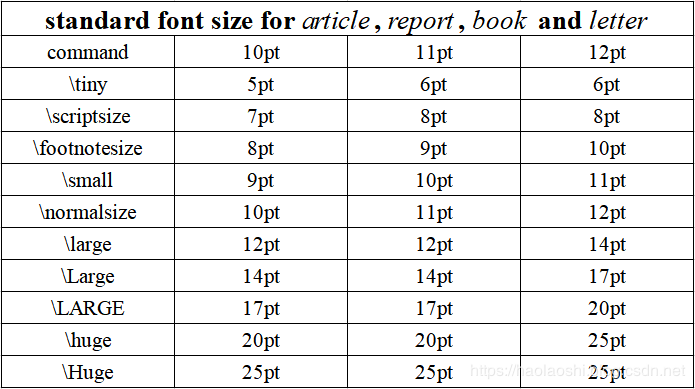
\includegraphics[width=\linewidth]{font.png}
	\caption{Figure in two column}
\end{figure}
(\cite{duchovn2014path})

\begin{figure}
	\centering
	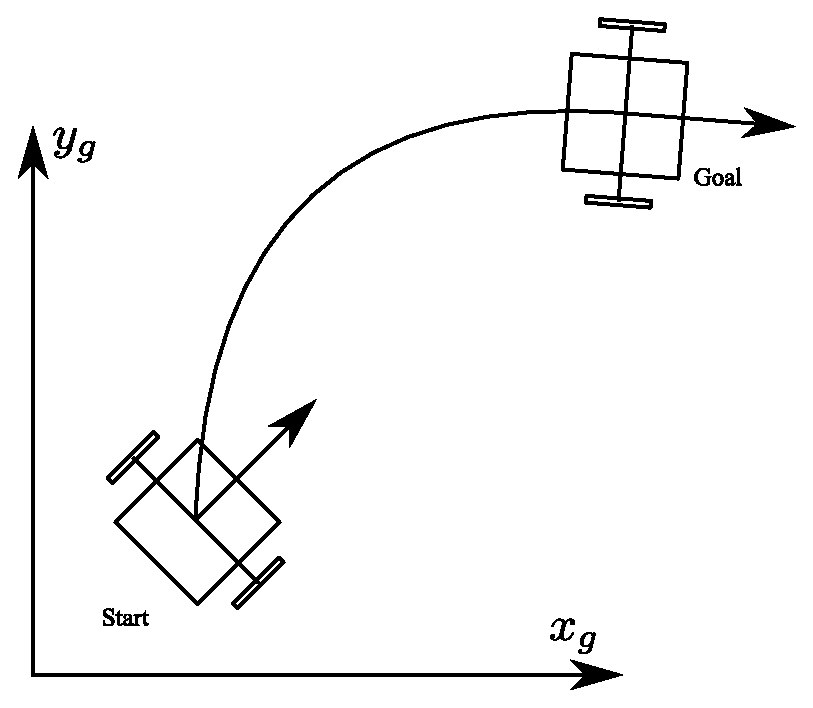
\includegraphics[width=0.7\linewidth]{ddtest.eps}
	\caption{import eps file from inkscape}
\end{figure}

%%--------------------------------------------------------------------------------








%%---------------------------------------------------------------------------------
\section{RESULT AND DISCUSSION}
Results should be discussed thoroughly in this section, if necessary with the aid of figures and tables. The tables and figures should fit within column width of 8.52 cm.
Table 1. Sample of table format (\cite{al2015multiple})

\begin{table}
	\begin{center}
		\caption{Extended Kalman Filter Algorithm}
		\label{Table: Extended Kalman Filter Algorithm}
		\begin{tabular}{lll}
			\hline
			Prediction&&  \\
			\hline
			State estimate&& \(\hat{X}^-_k = f(\hat{X}^-_{k-1},u_{k-1})\) \\
			error co-variance&& \(P^-_k = F_{k-1}P^+_{k-1}F^T_{k-1} + Q\)\\
			\hline
			Correction&&  \\
			\hline
			residual&& \(\tilde{y}_k = Z_k - h(\hat{X}^-_k)\)\\
			Kalman Gain&& \(K_k = P^-_kH^T_k(R+H_kP^-_kH^T_k)^{-1}\)\\
			state estimate&& \(\hat{X}^+_k = \hat{X}^-_k + K_k\tilde{y}\)\\
			error co-variance&& \(P^+_k = (I-K_kH_k)P^-_k\)\\
			\hline 
		\end{tabular}
	\end{center}
\end{table}

Energy Resource Emission Factor
(t CO2/TJ) Available Resource (TJ)  Coal 105 600,000  Oil 75 800,000  Natural Gas  55 200,000  Others 0 >400,000  Total  >2,000,000  
Fig.1. Captions should be provided as well
References should be cited using this format (Wooly et al., 2000; Ahmad, 2002). They should be listed at the end of the paper in alphabetical order.
%%---------------------------------------------------------------------------------









%%---------------------------------------------------------------------------------
\section{CONCLUSIONS}
This section must summarize the key findings of the study and describe potential areas for further research.
%%---------------------------------------------------------------------------------









%%---------------------------------------------------------------------------------
\section*{ACKNOWLEDGMENT}
You may place your acknowledgments here. Write only essential acknowledgments.\\
\blindtext \blindtext \blindtext \blindtext \blindtext \blindtext \blindtext \blindtext 
%%---------------------------------------------------------------------------------



%%---------------------------------------------------------------------------------
\printbibliography[title={REFERENCES}]

%%---------------------------------------------------------------------------------
\end{document}